\documentclass[12pt,english]{article}
\usepackage{geometry}
\geometry{verbose,letterpaper,tmargin=2.4cm,bmargin=2.4cm,lmargin=2.4cm,rmargin=2.4cm}
\usepackage[T1]{fontenc}
\usepackage{lmodern}
\usepackage{amssymb,amsmath}
\usepackage{ifxetex,ifluatex}
\usepackage{natbib}
\bibliographystyle{plainnat}
\usepackage{graphicx}
\usepackage{caption}
\usepackage{subcaption}
\usepackage{brush_style}
\usepackage{setspace}
\usepackage{lineno}
\begin{document}


\appendix
\section{Appendix}
In Appendix \ref{stab}, we provide the details for assessing the persistence of a population with an integrodifference model and we discuss the effect of the harvesting function on population persistence.  In Appendix \ref{sep}, we provide the details for assessing population persistence with separable dispersal kernels.  In Appendix \ref{gausapp} and \ref{sinapp}, we derive expressions for the critical harvesting rate and rate of environmental shift for Gaussian and sinuosoidal dispersal kernels.  In Appendix \ref{approxcrit}, we derive approximate expressions for these critical rates.

\subsection{Determining stability \label{stab}}
As in Zhou et al. \citep{ZhouKot2011}, let $k(x-y)$ be a dispersal kernel, let $f(n)$ be a recruitment function, and let $g(n)$ be the harvesting function describing the number of adults harvested from a population of size $n$.  The integrodifference model describing the population over time is given by 

\begin{equation} n_{t+1}(x)=\int_{-L/2+ct}^{L/2+ct}k(x-y)f(n_t(y)-g(n_t(y)))dy. \label{integro} \end{equation}

To find a traveling pulse, we are only interested in the population density as a function of the location within the patch rather than absolute position, $\overline{x}\equiv x-ct$.

\begin{equation*}
n^*(\overline{x})\equiv n^*(x-ct)=n_t(x).   \label{trav} 
\end{equation*}

The integrodifference equation (\ref{integro}) gives us an expression for $n^*$:

\begin{align}
n^*(\overline{x}-c)&=\int_{-L/2}^{L/2}k(\overline{x}-\overline{y})f(n^*(\overline{y})-g(n^*(\overline{y})))d\overline y \notag
\\ \Rightarrow n^*(\overline{x})&=\int_{-L/2}^{L/2}k(\overline{x}+c-\overline{y})f(n^*(\overline{y})-g(n^*(\overline{y}))d\overline y  \label{pulse}
\end{align}
As long as $f(0)=0$, there is a trivial solution to this problem where $n^*(\overline{x})\equiv 0$ for all $\overline{x}\in[-L/2,L/2]$, i.e. there is a trivial traveling pulse with no fish in it.  If the trivial traveling pulse is unstable, even very small populations will persist or grow and avoid crashing back to the trivial pulse.  To evaluate the stability of a traveling pulse, we introduce a small perturbation to the traveling pulse $n^*(\overline{x})$ and see if this perturbation grows or shrinks over time:

\begin{align}
n_t(x)&=n^*(\overline{x})+\xi_t(x) \notag
\\ \Rightarrow \xi_{t+1}(x)&=n_{t+1}(x)-n^*(\overline{x}) \notag
\\ \Rightarrow \xi_{t+1}(x)&=\int_{-L/2+ct}^{L/2+ct}k(x-y)\big(f(n_t(y)-g(n_t(y)))-f(n^*(\overline{y})-g(n^*(\overline{y}))\big)dy \text{ using (\ref{pulse})} \notag
\\ \Rightarrow \xi_{t+1}(x)&=\int_{-L/2+ct}^{L/2+ct}k(x-y)(1-g'(n^*(\overline{y})))f'(n^*(\overline{y})-g(n^*(\overline{y}))\xi_t(y)dy \notag
\\& \text{ by linearizing around the traveling pulse} \notag
\\ \Rightarrow \xi_{t+1}(x)&=\int_{-L/2+ct}^{L/2+ct}k(x-y)(1-g'(0))f'(0)\xi_t(y)dy \text{ if $n^*(\overline{x})=0$} \label{perturb}
\end{align}


If we assume $\xi_t(x)=\lambda^tu(x-ct)$ for some $\lambda\in\R$ and $u:[-L/2,L/2]\to\R$, then the perturbation grows in time if and only if $\lambda >1$.  Using Equation (\ref{perturb}), we can rewrite $\xi_{t+1}(x)$,
\begin{align*}
\lambda u(x-ct-c)&=(1-g'(0))f'(0)\int_{-L/2+ct}^{L/2+ct}k(x-y)u(y-ct)dy
\\ \\\Rightarrow \lambda u(\overline{x})&=(1-g'(0))f'(0)\int_{-L/2}^{L/2}k(\overline{x}+c-\overline{y})u(\overline{y})dy
\end{align*}

Define the integral operator
$$ \psi_f(u)(x)=(1-g'(0))f'(0)\int_{-L/2}^{L/2}k(x+c-y)u(y)dy. $$
Then the perturbation to the traveling pulse will satisfy 
\begin{equation} \psi_f(u)(x)=\lambda u(x) \label{eigen} \end{equation}
$\lambda$ and $u$ are thus an eigenvalue and eigenvector of the functional operator $\psi_f$.  The trivial traveling pulse is unstable when the dominant eigenvalue of $\psi_f$ is greater than $1$.


The biomass in the equilibrium traveling wave depends on the specific functional form of the harvesting function $g(n)$.  However, the persistence of the population only depends on $g'(0)$ so in this paper, we only considered a proportional harvesting function, i.e. the amount of fish harvested obeyed $g(n)=hn$.  For this function, $g'(0)=h$.  

\subsection{Separable dispersal kernels \label{sep}}
Jentzsch's theorem shows that there is an eigenfunction $u$, provided that the kernel $k$ satisfies some properties \citep{ZhouKot2011}.  Finding the eigenfunctions and eigenvalues is in general a hard problem to solve.  It becomes easier if the kernel $k$ is separable, i.e. there are functions $a_n,b_n$ such that $k(x-y)=\sum_{n=1}^\infty a_n(x)b_n(y)$.  In that case, (\ref{eigen}) becomes
\begin{align}
\lambda u(x)&=f'(0)\sum_{n=1}^\infty\left( a_n(x)\int_{-L/2}^{L/2}b_n(y-c)u(y)dy\right) \notag
\\ \Rightarrow \lambda\int_{-L/2}^{L/2}b_k(x-c)u(x)dx&=f'(0)\sum_{n=1}^{\infty}\left(\int_{-L/2}^{L/2}b_n(x-c)u(x)dx\right)\left(\int_{-L/2}^{L/2}a_n(y)b_k(y-c)dy\right) \notag
\\ \Rightarrow \lambda d_k&=f'(0)\sum_{n=1}^\infty A_{nk}d_n  \label{problem}
\end{align}
where
\begin{equation*}
A_{nk}=\int_{-L/2}^{L/2}a_n(x)b_k(x-c)dx \text{ and } d_k=\int_{-L/2}^{L/2}b_k(x-c)u(x)dx
\end{equation*}
Finding the eigenvalues of (\ref{eigen}) then reduces to finding the eigenvalues of the matrix $(A_{nk})_{n,k=1}^\infty$.

\subsection{Gaussian dispersal kernel \label{gausapp}}
The Gaussian dispersal kernel is given by
$$k(x-y)=\frac{1}{2\sqrt{D\pi}}e^{\frac{-(x-y)^2}{4D}}.$$
As in \citep{Latore:1998fk}, this separable kernel can be written as
$$k(x-y)=\sum_{n=0}^\infty a_n(x)b_n(y)$$
where
$$a_n(x)=b_n(x)=\frac{1}{\sqrt{2n!\sqrt{D\pi}}}e^{-x^2/4D}\left(\frac{x}{\sqrt{2D}}\right)^n.$$

As a first approximation to $k$ we ignore all but the $0^{th}$ terms for $a_n$ and $b_n$ so that Equation (\ref{problem}) becomes
\begin{align*}
\lambda d_0(c)&=(1-h)f'(0)A_{00}(c)d_0(c)
\\ \Rightarrow \lambda&=(1-h)R_0A_{00}(c)
\\\text{ where } A_{00}(c)&=2\sqrt{2}\exp\left(\frac{-c^2}{8D}\right)\left[\text{erf}\left(\frac{L-c}{2\sqrt{2D}}\right)-\text{erf}\left(\frac{-L-c}{2\sqrt{2D}}\right)\right]
\end{align*}
where $\text{erf}$ is the error function.  The critical rate of environmental shift $c^*$ and the critical harvesting rate $h^*$ are those values of $c$ and $h$, respectively, that make $\lambda=1$.

\subsection{Sinusoidal dispersal kernel \label{sinapp}}
A sinusoidal dispersal kernel is given by 
$$k(x-y)=\left\{\begin{array}{ccccc}
\frac{w}{2}\cos(w(x-y)) & , & |x-y|\leq\frac{\pi}{2w}
\\ 0 & , & |x-y|>\frac{\pi}{2w}
\end{array}\right.
$$
where $L$ is the length of the patch and we assume $\frac{\pi}{2w}>L,c<\frac{\pi}{2w}-L$.

In this case, $k(x-y)=\frac{w}{2}\cos(wx)\cos(w(y-c))+\frac{w}{2}\sin(wx)\sin(w(y-c))$ so that $A_{ij}$ and $d_i$ can be found for $i,j=1,2$ and (\ref{problem}) reduces to 
$$\lambda^2-\left(\frac{R_0(1-h)wL}{2}\cos(wc)\right)\lambda+\frac{R_0^2(1-h)^2}{16}\left(w^2L^2-\sin^2(wL)\right)=0.$$

If we solve for $\lambda$,we find
\begin{equation*} \lambda=(1-h)R_0\left[\frac{wL\cos(wc)}{4}+\frac{1}{4}\sqrt{\sin^2(wL)-w^2L^2\sin^2(wc)}\right]. \label{cosine} \end{equation*}


Zhou et al. \citep{ZhouKot2011} solve for the critical speed, $c^*$, at which the population will be driven extinct:
$$c^*=c^*(R_0)=\frac{1}{w}\cos^{-1}\left[\frac{16+R_0^2(1-h)^2(w^2L^2-\sin^2(wL))}{8R_0(1-h)wL}\right].$$
Similarly, we can solve for the critical harvesting rate, $h^*$, at which the population will be driven extinct:
$$
h^*=1-\frac{1}{R_0}\cdot\frac{4wL}{w^2L^2-\sin^2(wL)}\left[\cos(wc)-\sqrt{\cos^2(wc)-1+\frac{\sin^2(wL)}{w^2L^2}}\right] 
$$

\subsection{Approximate critical harvesting proportions \label{approxcrit}}
~\\We will use the following Taylor series to make approximations of the critical harvesting proportions under the two dispersal kernels:
\begin{align*}
\cos(x)&=1-\frac{x^2}{2}
\\ \cos^2(x)&=1-x^2
\\ \sin^2(x)&=x^2-\frac{x^4}{3}
\\ erf(x)&=\frac{2}{\sqrt{\pi}}(x-\frac{x^3}{3})
\\ \exp(x)&=1+x+\frac{x^2}{2}
\end{align*}
For the sinusoidal kernel we found 
\begin{equation}
h^*=1-\frac{1}{R_0}\cdot\frac{4wL}{w^2L^2-\sin^2(wL)}\left[\cos(wc)-\sqrt{\cos^2(wc)-1+\frac{\sin^2(wL)}{w^2L^2}}\right] 
\end{equation} 
Using the Taylor series and the fact that $w=\frac{\sqrt{\frac{\pi^2}{4}-2}}{\sigma}$ where $\sigma^2$ is the variance of the sinusoidal kernel,
\begin{align*}
h^*&\sim 1-\frac{1}{R_0}\cdot\frac{12wL}{w^4L^4}\left[1-\frac{w^2c^2}{2}-\sqrt{1-w^2c^2-\frac{w^2L^2}{3}}\right]
%\\&=1-\frac{1}{R_0}\cdot\frac{12}{w^3L^3}\left[1-\frac{w^2c^2}{2}-\sqrt{1-w^2c^2-\frac{w^2L^2}{3}}\right]
%\\&=1-\frac{1}{R_0}\cdot\frac{12\sigma^3}{L^3(\frac{\pi^2}{4}-2)^{3/2}}\left[1-\frac{(\frac{\pi^2}{4}-2)c^2}{2\sigma^2}-\sqrt{1-\frac{(\frac{\pi^2}{4}-2)c^2}{\sigma^2}-\frac{(\frac{\pi^2}{4}-2)L^2}{3\sigma^2}}\right]
%\\&=1-\frac{1}{R_0}\cdot\frac{6\sigma}{L^3(\frac{\pi^2}{4}-2)^{3/2}}\left[2\sigma^2-(\frac{\pi^2}{4}-2)c^2-\frac{2}{\sqrt{3}}\sigma\sqrt{3\sigma^2-(\frac{\pi^2}{4}-2)3c^2-(\frac{\pi^2}{4}-2)L^2}\right]
%\\&=1-\frac{1}{R_0}\cdot\frac{6\sigma}{L^34(\frac{\pi^2}{4}-2)^{3/2}}\left[8\sigma^2-(\pi^2-8)c^2-\frac{4}{\sqrt{3}}\sigma\sqrt{12\sigma^2-(\pi^2-8)3c^2-(\pi^2-8)L^2}\right]
%\\&=1-\frac{12}{R_0L^3(\pi^2-8)^{3/2}}\cdot\sigma\left[8\sigma^2-(\pi^2-8)c^2-\frac{4}{\sqrt{3}}\sigma\sqrt{12\sigma^2-(\pi^2-8)3c^2-(\pi^2-8)L^2}\right]
\\&=1-\frac{1}{R_0}\cdot\frac{4\sqrt{3}}{L^3(\pi^2-8)^{3/2}}\cdot\sigma\left[8\sqrt{3}\sigma^2-(\pi^2-8)\sqrt{3}c^2-4\sigma\sqrt{12\sigma^2-(\pi^2-8)(3c^2+L^2)}\right]
\end{align*}
For the Gaussian kernel we found 
\begin{equation}
h^*=1-\frac{2\sqrt{2}\exp\left(\frac{c^{2}}{8D}\right)}{R_0\left[erf\left(\frac{L-c}{2\sqrt{2D}}\right)-erf\left(\frac{-L-c}{2\sqrt{2D}}\right)\right]}
\end{equation} 
Using the Taylor series and the fact that $D=\frac{\sigma^2}{2}$ where $\sigma^2$ is the variance of the exponential kernel,
\begin{align*}
h^*&\sim 1-\frac{\sqrt{2\pi}(1+\frac{c^2}{8D}+\frac{c^4}{128D^2})}{R_0\sqrt{\pi}\left[\frac{L-c}{2\sqrt{2D}}-\frac{(L-c)^3}{3(2\sqrt{2D})^3}-\frac{-L-c}{2\sqrt{2D}}+\frac{(-L-c)^3}{3(2\sqrt{2D})^3)}\right]}
%\\&= 1-\frac{\sqrt{2\pi}(1+\frac{c^2}{8D}+\frac{c^4}{128D^2})}{R_0\left[\frac{2L}{2\sqrt{2D}}+\frac{-L^3+3L^2c-3Lc^2+c^3-L^3-3L^2c-3Lc^2-c^3}{3(2\sqrt{2D})^3}\right]}
%\\&= 1-\frac{\sqrt{2\pi}(1+\frac{c^2}{8D}+\frac{c^4}{128D^2})}{R_0\left[\frac{L}{\sqrt{2D}}-2\frac{L^3+3Lc^2}{3(2\sqrt{2D})^3}\right]}
%\\&= 1-\frac{\sqrt{2\pi}(1+\frac{c^2}{8D}+\frac{c^4}{128D^2})}{R_0L\left[\frac{48D-2(L^2+3c^2)}{3(2\sqrt{2D})^3}\right]}
%\\&= 1-\frac{3*32D\sqrt{D\pi}(1+\frac{c^2}{8D}+\frac{c^4}{128D^2})}{R_0L\left(48D-2(L^2+3c^2)\right)}
%\\&= 1-\frac{3*32D\sqrt{D\pi}(\frac{128D^2+16c^2D+c^4}{128D^2})}{R_0L\left(48D-2(L^2+3c^2)\right)}
%\\&= 1-\frac{3\sqrt{\pi}(128D^2+16c^2D+c^4)}{4R_0L\sqrt{D}\left(48D-2(L^2+3c^2)\right)}
%\\&= 1-\frac{3\sqrt{2\pi}(32\sigma^4+8c^2\sigma^2+c^4)}{4R_0L\sigma\left(24\sigma^2-2(L^2+3c^2)\right)}
\\&= 1-\frac{1}{R_0}\cdot\frac{3\sqrt{2\pi}}{8L}\frac{(32\sigma^4+8c^2\sigma^2+c^4)}{\sigma\left(12\sigma^2-(L^2+3c^2)\right)}
\end{align*}
In the case of both kernels, the critical harvesting proportion can be approximated by a function that looks like 
\begin{equation}
h^*\sim1- \frac{1}{R_0}\cdot C(L)f(\sigma^2,c^2,L^2+3c^2)
\end{equation}
where $C(L,R_0)$ is a decreasing function of the length of the viable patch and the intrinsic growth rate.

\subsection{MPA fluctuations}

\begin{figure}
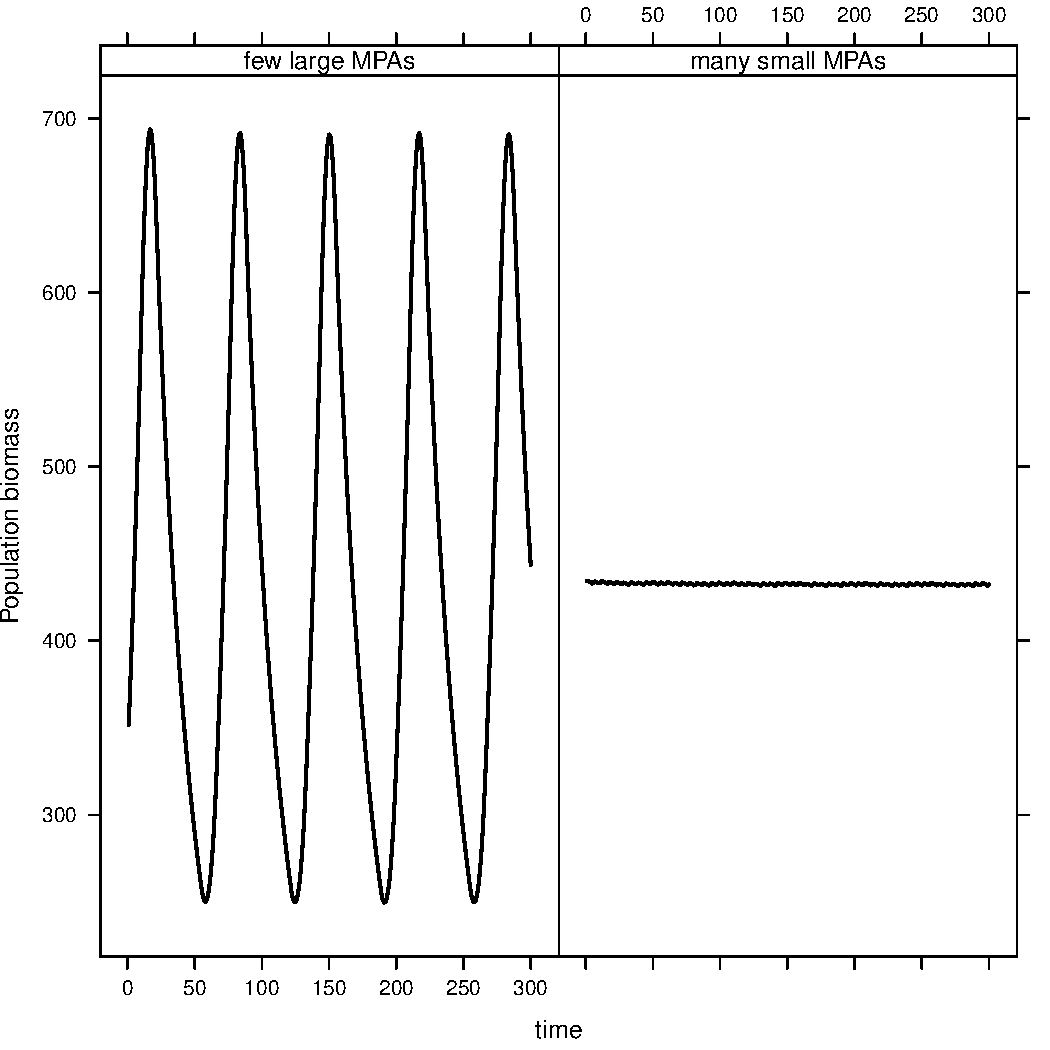
\includegraphics[width=1\textwidth]{plots/bounded_flux.pdf}
\caption{Comparing population over time where $s = 0.1, h = 0.08$, see bounded\_flux.R for code that made this plot. }
\end{figure}

\bibliography{fish}

\end{document}